% Preview of the "six modes move together" sketch, at poster size (left column, ~15 cm).
% Same font, colours and car as the attack-scenario figure in poster.tex.
\documentclass[tikz,border=6pt]{standalone}
\usepackage{helvet}
\renewcommand{\familydefault}{\sfdefault}
\usetikzlibrary{arrows.meta}

\definecolor{cleanC}{HTML}{2563B0}
\definecolor{attackC}{HTML}{EB6834}
\definecolor{truthC}{HTML}{2E8B57}
\definecolor{modeC}{HTML}{8C8C8C}

% Top view of a car heading +x, centred at (#1, #2)
\newcommand{\topcar}[2]{%
	\begin{scope}[shift={(#1, #2)}]
		\draw[fill=white, line width=1.2pt, rounded corners=5pt] (-0.8, -0.36) rectangle (0.8, 0.36);
		\fill[black!55, rounded corners=2pt] (0.22, -0.28) rectangle (0.48, 0.28);
		\fill[black!55, rounded corners=2pt] (-0.68, -0.25) rectangle (-0.52, 0.25);
	\end{scope}}

% Six predicted futures from the car front (3, 0), the whole fan rotated by #1 degrees
\newcommand{\fan}[1]{%
	\begin{scope}[rotate around={#1:(3.0, 0)}]
		\foreach \e in {1.2, 0.9, 0.6, 0.3, 0.0, -0.3}
			\draw[modeC, line width=1.8pt, dash pattern=on 6pt off 4pt]
				(3.0, 0) .. controls (4.6, 0) and (5.6, {0.8*\e}) .. (7.0, \e);
	\end{scope}}

\begin{document}
\fontsize{13.5}{16}\selectfont
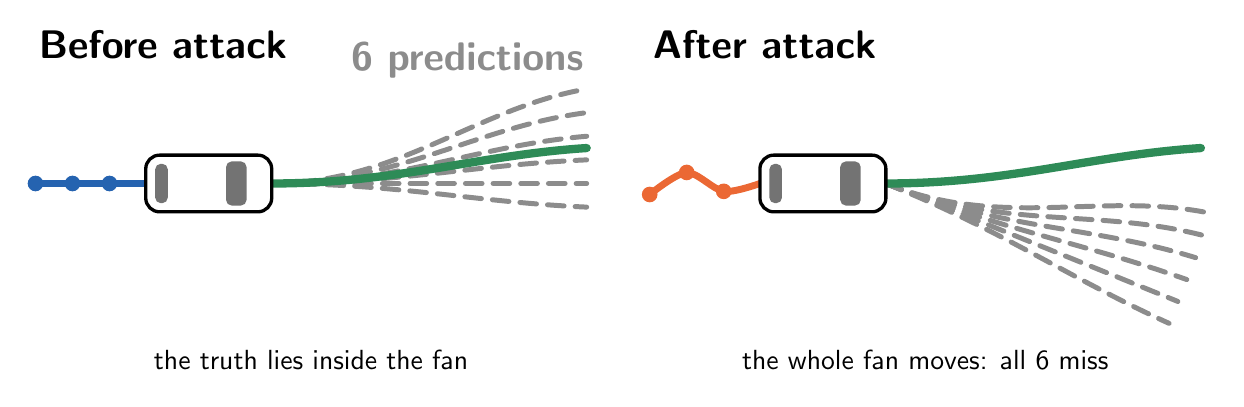
\begin{tikzpicture}[line cap=round,
	dot/.style={circle, fill, inner sep=2pt},
	lab/.style={font=\fontsize{13.5}{16}\selectfont\bfseries, inner sep=1pt}]

	% --- before the attack: the truth lies inside the fan
	\node[anchor=south west, lab] at (0, 1.55) {Before attack};
	\draw[cleanC, line width=2.5pt] (0, 0) -- (1.4, 0);
	\foreach \x in {0, 0.47, 0.94} \node[dot, cleanC] at (\x, 0) {};
	\fan{0}
	\draw[truthC, line width=3pt] (3.0, 0) .. controls (4.6, 0) and (5.6, 0.36) .. (7.0, 0.45);
	\topcar{2.2}{0}
	\node[anchor=south east, font=\fontsize{13.5}{16}\selectfont\bfseries, text=modeC, inner sep=1pt] at (7.0, 1.3) {6 predictions};
	\node[anchor=north, align=center] at (3.5, -2.0) {the truth lies inside the fan};

	% --- after the attack: same fan, shifted as a whole; the truth is outside
	\begin{scope}[xshift=7.8cm]
		\node[anchor=south west, lab] at (0, 1.55) {After attack};
		\draw[attackC, line width=2.5pt] plot[smooth] coordinates {(0, -0.14) (0.47, 0.14) (0.94, -0.1) (1.4, 0)};
		\foreach \x/\y in {0/-0.14, 0.47/0.14, 0.94/-0.1} \node[dot, attackC] at (\x, \y) {};
		\fan{-22}
		\draw[truthC, line width=3pt] (3.0, 0) .. controls (4.6, 0) and (5.6, 0.36) .. (7.0, 0.45);
		\topcar{2.2}{0}
		\node[anchor=north, align=center] at (3.5, -2.0) {the whole fan moves: all 6 miss};
	\end{scope}

\end{tikzpicture}
\end{document}
